%----------------------------------------------------------------------------------------
%	PACKAGES AND OTHER DOCUMENT CONFIGURATIONS
%----------------------------------------------------------------------------------------

\documentclass[fleqn,11pt]{SelfArx} % Document font size and equations flushed left

\usepackage{parskip}
\usepackage{microtype}
\usepackage{svg}
\usepackage{float}
\usepackage{placeins}
\usepackage[english]{babel} % Specify a different language here - english by default
\usepackage{listings}
\usepackage{fontspec}
\usepackage{hyperref}
\usepackage{amsmath}
% \usepackage{lipsum} % Required to insert dummy text. To be removed otherwise
\setmainfont{TeX Gyre Termes}
%----------------------------------------------------------------------------------------
%	COLUMNS
%----------------------------------------------------------------------------------------

\setlength{\columnsep}{0.55cm} % Distance between the two columns of text
\setlength{\fboxrule}{1pt} % Width of the border around the abstract

%----------------------------------------------------------------------------------------
%	COLORS
%----------------------------------------------------------------------------------------

\definecolor{color1}{RGB}{124,0,0} % Color of the article title and sections
\definecolor{color2}{RGB}{150,150,150} % Color of the boxes behind the abstract and headings

%----------------------------------------------------------------------------------------
%	HYPERLINKS
%----------------------------------------------------------------------------------------

\usepackage{hyperref} % Required for hyperlinks
\hypersetup{hidelinks,colorlinks,breaklinks=true,urlcolor=color2,citecolor=color1,
  linkcolor=color1,bookmarksopen=false,pdftitle={Title},pdfauthor={Author}}

%----------------------------------------------------------------------------------------
%	ARTICLE INFORMATION
%----------------------------------------------------------------------------------------

\PaperTitle{
    HAMdetector: Combining information to detect HLA-associated mutations with a
    Bayesian regression model
} % Article title

\Authors{Daniel Habermann\textsuperscript{1}, ..., Daniel Hoffmann\textsuperscript{1}} % Authors
\affiliation{\textsuperscript{1}\textit{Bioinformatics \& Computational Biophysics, Faculty of Biology, University of Duisburg-Essen, 45117 Essen, Germany}} % Author affiliation
% \affiliation{\textsuperscript{2}\textit{Department of Chemistry, University of Examples, London, United Kingdom}} % Author affiliation
% \affiliation{*\textbf{Corresponding author}: john@smith.com} % Corresponding author

\Keywords{human leukocyte antigen system, HLA, multiple sequence alignment, escape mutations, 
  viral escape, Bayesian inference, sparsity, horseshoe, epitope prediction} % Keywords - if you don't want any simply remove all the text between the curly brackets
\newcommand{\keywordname}{Keywords} % Defines the keywords heading name

%----------------------------------------------------------------------------------------
%	ABSTRACT
%----------------------------------------------------------------------------------------

\Abstract{
  \\
  \textbf{Motivation} \\
  The human leukocyte antigen system (HLA) is of paramount importance to combat viral infections by presenting peptides on the cell surface via MHC I. Thus, CD8+ cytotoxic T-Lymphocytes exert a strong selection pressure towards virus variants that escape that immune recognition pathway, e.g. through point mutations that decreases binding of the respective peptide to MHC I. \\

  Reliably identifying HLA-associated mutations is important for understanding viral evolution, but experimental methods like binding assays are prohibitively expensive for large-scale use and fail to recognize other mechanisms of immune escape like proteasomal processing.

  One step in finding these mutations is through the statistical analysis of sequence data. However, existing methods are based on null hypothesis significance testing and do not make use of all the available information and therefore have unsatisfactory real-world performance. \\

  \textbf{Results} \\
  Here, we present a Bayesian regression model that is easily extensible to include information from different sources (e.g. epitope prediction software) and makes use of recent advances in Bayesian inference, e.g. by using a sparsifying prior. We show that including this kind of information improves predictive performance considerably over state-of-the-art methods. \\

  \textbf{Availability and Implementation} \\
  The source code of this software is available at \url{http://github.com} under a permissive MIT license. \\

  \textbf{Supplementary information} \\
  \href{https://google.com}{Supplementary data} are available at \textit{Bioinformatics} online. \\
}

%----------------------------------------------------------------------------------------
\begin{document}

\flushbottom % Makes all text pages the same height

\maketitle % Print the title and abstract box

{
  \hypersetup{linkcolor=black}
  \tableofcontents
}


\section{Introduction}

\subsection{The HLA system}

One way how the human immune system is able to recognize intracellular viral infections is through the human leukocyte antigen system\nolinebreak\cite{Germain1994}: In cells with active protein biosynthesis, proteins are continuously synthesized and also degraded by a process called proteasomal degradation, which cleaves proteins into linear peptides of varying length\nolinebreak\cite{Goldberg2002}.

A small subset of these peptides is presented on the cell surface via receptors called MHC class I (HLA-A, HLA-B and HLA-C in humans). The genomic region encoding for MHC I is known to be highly polymorphic, with more than 20000 different HLA alleles described today\nolinebreak\cite{Robinson2014}. The resulting gene products differ in their binding properties, which means that cells from different individuals present a highly diverse set of peptides on their surface.

Cytotoxic T cells are selected during maturation to only weakly bind to peptide/MHC I complexes when the peptide originated from proteins of the usual proteome, but might be able to strongly bind to complexes of MHC I with peptides which are  generated from of a viral protein\nolinebreak\cite{Murata2007}. Upon activation, T cells induce cytolytic activity and recruit other immune cells \nolinebreak\cite{Harty2000}.

\subsection{HLA escape}
In this way, the HLA system exerts strong selection pressure towards virus variants that escape T cell recognition\nolinebreak\cite{Borrow1997}, for example through a point mutation that results in reduced binding of an immunogenic peptide to MHC I or through a set of mutations that alters the viral protein in such a way that it is cleaved into different peptides that are not recognized by the host's T cell repertoire\nolinebreak\cite{Yewdell2002}.

The evolutionary events are complex and occur not only on the level of individuals, where a virus adapts to specific features of the host, but also on the population level, because HLA alleles differ in their frequency across geographic regions\nolinebreak\cite{Kawashima2009}. Upon transmission to a new host, HLA escape mutations can revert to their wild type, as HLA escape mutations are associated with a reduction in viral replicative capacity\nolinebreak\cite{Matthews2008}. Kawashima et al. \nolinebreak\cite{Kawashima2009} describe an escape mutation that is selected by HLA allele HLA-B*51, does not strongly affect viral replicative capacity, and therefore slowly enriches over time in Japan, where HLA-B*51 commonly occurs.

How quickly a given escape mutation is selected upon transmission in a host depends on the magnitude of the reduction in viral replicative capacity, on the strength of selection pressure, and also on the genetic background, e.g. some escape mutations require compensatory mutations which partly attenuate the negative impact on viral replicative capacity.

Studying HLA escape provides a unique opportunity to gain insight into viral evolution, on the host level, but also on the population level.
Unfortunately, identifying HLA escape mutations is difficult in practice.

\subsection{Identifying HLA-escape mutations}

There are several experimental methods available to study HLA escape: Recombinant MHC-I molecules can be used in binding assays. Upon complex formation with a peptide, a change in conformation can be detected with conformation-specific antibodies. This method is relatively fast, but only measures binding affinity of a peptide to MHC-I and does not account for antigen processing or immunodominance, which describes the observation that a peptide may be presented via MHC-I on the cell  surface, but does not induce an immune response.

An experimental setup that resembles the conditions in-vitro more closely but is also more time-consuming is to measure CD8+ T cell responses instead. This is usually done by stimulating peripheral blood mononuclear cells with prototype and variant peptides and measuring the secretion of IFN-\gamma{} by intracellular cytokine staining and fluorescence-assisted cell sorting.

To analyze CD8+ T cell responses against endogenously processed antigens, it is necessary to generate cell-lines stably expressing the antigen in question and adding antigen-specific CD8+ T cells. This method scales poorly as it requires transfection of cell lines and antigen-specific expansion of CD8+ T cells.

\subsection{Computational methods}

Because the currently available experimental methods do not scale well enough to analyze whole viral genomes, a useful strategy might be to use annotated sequence data to identify candidate HLA escape mutations that can then be verified experimentally.

As the selection pressure exerted by cytotoxic T cells depends on successful recognition of viral peptides on the cell surface, escape mutations are often HLA-allele specific and can therefore be detected as HLA-allele dependent footprints in sequence alignments of viral proteins\nolinebreak\cite{Moore2002}: At certain alignment positions, a replacement might be more frequently observed in sequences from hosts with a specific HLA allele than in  sequences from hosts without that HLA allele. By quantifying this difference for all replacement and HLA allele pairs, it is possible to identify replacements that are enriched in sequences coming from hosts with certain HLA alleles, and thus are likely to be HLA escape mutations.

One way of quantifying this enrichment is Fisher's exact test\nolinebreak\cite{Fisher1922}: For a given replacement \(R_{i}\) at alignment position \(i\) and HLA allele \(H\), a 2-by-2 contingency table is constructed containing the absolute counts of the number of sequences in the four possible categories  (\(R_{i}\), \(H\)), (\(R_{i}\), \(!H\)), (\(!R_{i}\), \(H\)) and (\(!R_{i}\), \(H\)), where \(!R_{i}\) denotes any replacement except \(R_{i}\), and \(!H\) denotes any HLA allele except \(H\).

Fisher's exact test is a conventional null hypothesis significance test (NHST) that generates p-values. In this case, the null hypothesis is that HLA allele \(H\) and  replacement \(R_{i}\) are independent, and the p-value is the probability of observing a deviation from independence that is at least as extreme as in the data at hand under the assumption that the null hypothesis is true.

Fisher's exact test has the advantage of being easy to apply\nolinebreak\cite{Budeus2016},  but also has several disadvantages that are outlined in Carlson et al.\nolinebreak\cite{Carlson2008}. The most striking one is that viral sequences share a common phylogenetic history, and,  therefore, treating sequences as independent and identically distributed samples may under- or overestimate effect sizes. In the context of hypothesis testing, this leads to increased false positive and false negative rates. 

Another issue of applying Fisher's exact test is that HLA class I loci are located in proximity on chromosome 6 and are therefore in linkage disequilibrium, which means that HLA alleles are not inherited completely independent of each other, i.e. inheritance of one HLA allele correlates with inheritance of another HLA allele. When using a statistical method that tests each HLA allele individually without considering the whole set of alleles present, spurious associations might occur: If HLA allele \(H_{1}\) is associated with an amino acid replacement \(R\), but \(H_{1}\) is in linkage disequilibrium with another allele \(H_{2}\), this also means that we observe an association between replacement \(R\) and \(H_{2}\), even in absence of any underlying escape mechanism.

Correlations can not only occur between HLA alleles, but also between replacements. This kind of codon covariation occurs for example in compensatory mutations that attenuate the negative impact of immune escape mutations. For instance, a compensatory mutation might lead to a conformational change in such a way that the mutated protein resembles the original wild type more closely.

Carlson et al. \nolinebreak\cite{Carlson2008} developed a method called  Phylogenetic Dependency Network that accounts for phylogenetic bias,  HLA linkage disequilibrium, and codon covariation and is based on null hypothesis significance testing.

\subsection{Issues with using p-values as a screening tool}

In addition to the aforementioned biological reasons why Fisher's exact test is  not suited for the analysis of sequence data, there are also more fundamental statistical issues that universally occur when using p-values as a screening tool\nolinebreak\cite{Amrhein2017}:

In the presence of small effect sizes and high variance between measurements, as  it is typically the case when working with biological data, statistically significant results can often be misleading and are likely to be in the wrong direction (a so-called type S error) or greatly overestimate an effect (a so-called type M error)\nolinebreak\cite{Gelman2014}. This problem has recently been widely appreciated in the literature in the context of the current \glqq replication crisis\grqq{}, which describes the circumstance that scientific claims with seemingly strong statistical evidence fail to replicate\nolinebreak\cite{Ioannidis2005}.

Another issue that occurs when using p-values as a screening tool is the problem of multiple comparisons. When applying a statistical test, the probability  of  obtaining a statistically significant result increases with each additional test, even in absence of any real effect. When using p-values as a filter, it is therefore likely to obtain significant effects that are in fact not real. To circumvent this problem, a common strategy is to control the false discovery rate, which is the expected proportion of false positives\nolinebreak\cite{Benjamini1995}. These adjustment procedures have the problem that, when performing many of such comparisons, none but the very largest effects remain.

Instead of performing many hypothesis tests and trying to adjust for them, we instead prefer to fit a single, multilevel model that contains all comparisons of interest. When using multilevel models, the problem of multiple comparisons can disappear entirely and  also yield more valid estimates\nolinebreak\cite{Gelman2012}.

\section{Material and methods}

When possible, we choose to fit Bayesian models. By using prior information, adding problem-specific structure and partial pooling, the accuracy of estimates can often be noticeably improved\nolinebreak\cite{Gelman2010}. Prior information does not necessarily mean to use external data, even a rough idea about the expected magnitude of estimates is often surprisingly effective.

Additionally, Bayesian statistics provides an accessible way to test models: By comparing data generated under the model's assumptions to the actually observed data, it is possible to identify important aspects of the dataset that the models fails to capture and subsequently improve the model until it is consistent with the observed data\nolinebreak\cite{Gabry2019}.

In the context of identifying HLA-associated mutations we propose to improve existing methods by the following additions, which can be broadly divided into  additional information and model structure:
\subsection*{Additional information}

  \textit{Binding affinity prediction}

    HLA-associated mutations are expected to lie more frequently in regions of known epitopes. There are vast experimental binding affinity data available of different peptides and MHC I molecule pairs, and there are well-established computational methods that use these data to extrapolate HLA binding for untested peptides. We show that, by including the outcome of these computational tools as input for a probabilistic model, the prediction of HLA-associated mutations can be improved.

  \textit{Antigen processing prediction}
  
    Similarly, there are also HLA-allele independent effects like antigen processing that influence presentation on MHC I. Second generational tools like MHCFlurry 2.0 use both binding affinity and antigen processing data to improve epitope prediction. For our tool HAMdetector, we use the output of MHCFlurry to benefit from this binding affinity and antigen processing data in order to predict HLA-associated mutations.

\subsection*{Model structure}

  \textit{Sparsity-inducing priors}
  
  Recent advantages in Bayesian inference include so-called sparsity-promoting priors. Sparsity-promoting priors convey the a priori expectation that most coefficients in a regression model are close to 0. This assumption also applies to HLA-associated mutations, because the number of epitopes that are restricted by a given HLA allele is typically small compared to the number of all possible epitopes. If no epitope spanning a given alignment position is presented on the MHC I molecule, any association between a replacement and the respective HLA allele  is likely to be due to random variation alone (or HLA linkage disequilibrium).
  
  It has been shown that using a sparsity-promoting prior when non-zero coefficients are sparse can drastically improve predictive performance, because the model is better able to differentiate between signal and noise.

  We show that a simple logistic regression model with a sparsity-promoting prior on the regression coefficients for the HLA alleles alone already performs roughly on-par  with the much more elaborate Phylogenetic Dependency Network approach from Carlson et al. when using the fraction of identified escapes that lie in known HLA epitopes as a benchmark.

  \textit{Partial pooling of 4-digit HLA alleles}
  
  It has recently been appreciated that binding specificities can vary drastically across  HLA alleles from the same allele group, e.g. between HLA-B*51:01 and HLA-B*51:03. For predicting HLA associated mutations, there has consequently been a shift to use 4-digit resolution data whenever available. This is not without downsides however, because overall, binding specificities are more similar for alleles in the same group, and, therefore, treating them as completely separate might unnecessarily fragment the available data.

  In Bayesian statistics, it is not required to chose one extreme or the other: Instead of either treating all HLA alleles from the same allele group as identical or as completely separate, partial pooling of the estimates allows something in between: By partial pooling, estimates do share some information across each other, but they are also allowed to vary if necessary.

  In the context of our model this means that observing a relevant association between a replacement and an HLA allele also makes the model more inclined to estimate relevant associations between that replacement and all other alleles from that allele group. The degree of this partial pooling can be estimated from the data, so if we do observe strong similarity of HLA alleles in a given allele group the estimates are more influenced by each other than if they do not.

\section{Implementation}

\subsection*{Model backbone}

We chose a logistic regression model as a backbone for two reasons: First, because it is easily extensible and secondly, because the coefficients are interpretable as expected increases on the log-odds scale, identical to the familiar interpretation of standard logistic regression models.
We also chose to fit the model in a Bayesian fashion using Stan, mostly because it allows us to make use of the hierarchical structure in the data and the possibility to use posterior predictive checks as a way of model checking.
Consider the following notation:

\begin{align}
  y_{ij} & \sim \text{bernoulli}(\theta_{ij}) \\
  \theta_{ij} & = \text{inv\_logit}(\beta_{0_{j}} + X_{i}\beta_{\text{HLA}_{j}})
\end{align}, 

where \(y_{ij}\) is the binary encoded observation at sequence \(i\) for replacement \(j\), \(\theta_{ij}\) is the estimated probability that we observe replacement \(j\) in sequence \(i\), \(X_{i}\) is the binary encoded (row) vector of HLA annotations for sequence \(i\), and \(\beta_{\text{HLA}_{j}}\) is the (column) vector of HLA regression coefficients for replacement \(j\) and  \(\text{inv\_logit}\) is the logistic link function. Note that, if we observe N different amino acid states at a certain alignment position, each of those are considered in turn to be the "replacement".

The regression coefficients \(\beta_{\text{HLA}_{j}}\) are the main focus of interest, as they quantify the association between the occurrence of replacement \(j\) and each of the observed HLA alleles. They are in units of log-odds, so a regression coefficient of somewhere around 2 means that when comparing sequences with and without that particular HLA allele, the log-odds of observing replacement \(j\) in presence of that HLA allele is increased by 2.

Reasoning about coefficients on the log-odds scale can sometimes be unintuitive. A useful approximation to interpret logistic regression coefficients on the probability scale is the so-called divide-by-4 rule, which means that a regression coefficient of 2 corresponds to an expected increase on the probability scale of about 2/4 = 50\%. 

\subsection*{Including phylogeny}

One problem that occurs when analyzing sequence data is that species share a common phylogenetic history. Standard statistical methods usually assume samples to be independent and identically distributed, which may lead to wrong conclusions when this assumption is strongly violated.
In the context of identifying HLA associations, Bhattacharya et al. demonstrated the importance of correcting for the phylogenetic structure.
There are many different approaches described in the literature for phylogenetic regression for binary dependent variables (see \cite{Ives2014}), where the most popular approach is to estimate an additional multivariate normally distributed intercept, where the covariance matrix is based on the branch lengths of a given phylogenetic tree \cite{Ives2009}.

This approach showed to be too computationally expensive to include in our model, so we chose a strategy that is similar to the one in Carlson et al. \cite{Carlson2008} for the Phylogenetic Dependency Network:

Consider a phylogenetic tree \(\Psi\) obtained from standard maximum likelihood methods for a given multiple sequence alignment. We are interested in estimating \(P(y_{ij}=1|\Psi)\), that is, the probability of observing the replacement \(j\) in sequence \(i\) based on the underlying phylogenetic model.
A quantity that can be readily computed using phylogenetic software like RAxML \cite{Stamatakis2014} is \(P(\Psi|y_{ij}=1)\). For this, we keep the tree topology fixed, annotate the tree with the binary observations \(y\) at its leaves and optimize the branch lengths. \(P(\Psi|y_{ij}=1)\) is then the likelihood of the annotated phylogenetic tree. We can then use Bayes' rule to invert that conditional probability by additionally computing \(P(\Psi|y_{ij}=0)\), which is done by altering the annotation for sequence \(i\) and keeping all other observations constant.

In order to check if the inferred probabilities \(P(y_{ij}=1|\Psi)\) faithfully reflect the observed data we use calibration plots (see fig.~\ref{fig:phylogeny-calibration}). All observations are binned according to their inferred probability \(P(y_{ij}=1|\Psi)\). If these probabilities are calibrated correctly, we expect that in a group of observations with an inferred probability \(P(y_{ij}=1|\Psi)\) of around x\% we really do observe \(y_{ij}=1\) around x\% percent of the time.

\begin{figure}[!ht]
  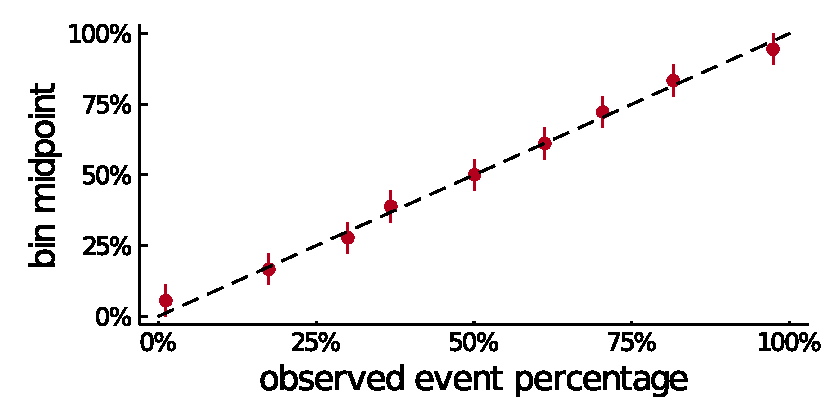
\includegraphics[width=1\linewidth]{plots/phylogeny_calibration.pdf}
  \caption{Calibration plot for the HBV dataset. For a description of all datasets used in this study see section~\ref{sec:results}. Calibration plots for the other datasets are shown in the appendix.
  All observations are first sorted by increasing estimated probability \(P(y_{ij}=1|\Psi)\) and then grouped into \(n\) bins.
  For each bin, the fraction of observations with \(y_{ij}=1\) (observed event percentage) is compared to the midpoint of each bin (the value in the center between the lowest and highest probability). The error bars show the cutpoints for each bin. If the probabilities are calibrated correctly, each dot is supposed to scatter closely around the diagonal line.}
  \label{fig:phylogeny-calibration}
\end{figure}

The estimated probabilities are then included in the model as additional intercepts:

\begin{equation}
\begin{aligned}
  y_{ij} & \sim \text{bernoulli}(\theta_{ij}) \\
  \theta_{ij} & = \text{inv\_logit}(\beta_{0_{j}} + \gamma~\text{logit}(P(y_{ij}=1|\Psi)) \\ + & X_{i}\beta_{\text{HLA}_{j}})
\end{aligned}
\end{equation}

The logit transform is used because is cancels out with the logistic link function. This means that the phylogeny information acts as a baseline in absence of any HLA effects. Note that we also include an additional parameter \(\gamma\), that is constrained to be positive. This helps because the inferred probabilities \(P(y_{ij}=1|\Psi)\) might not necessarily reflect the true underlying phylogenetic signal, for example because the phylogenetic tree does not match the observed data well enough.

A straight-forward extension of our model would be to also account for these sources of uncertainty, for example by using a Bayesian method to estimate a posterior distribution over possible tree topologies. The uncertainty over the tree topology and the underlying parameters of the phylogenetic model would then propagate into uncertainty of the estimated probabilities \(P(y_{ij}=1|\Psi)\). However, in order to not increase the runtime of the model further we  use standard maximum likelihood estimates and then include these in a way that allows for measurement error.

\subsection*{Including HLA linkage disequilibrium and codon covariation}

\begin{itemize}
  \item HLA linkage disequilibrium is accounted for by considering all HLA alleles of a sample at once.
  \item If strong correlations between HLA alleles: marginal posterior for both of them overlap with 0
  \item Codon covariation is not accounted for because we are mainly interested in HAMs.
  \item Model could be extended to include codon covariation by including them as additional predictors. This is possible because we use the horseshoe prior.
\end{itemize}

\subsection*{Including sparsity assumptions}

\begin{itemize}
  \item one of the recent advances in Bayesian inference: development of spacial priors to give model useful properties
  \item we expect most HLA coefficients to be 0, because no epitope spanning that region is presented on the cell surface, therefore no selection pressure and no association with possible replacements
  \item this is prior knowledge that should be incorporated in the model
  \item leads to better inferences because uncertainty of the regression coefficients does not propagate into observations.
  \item works by placing most probability mass very close to 0, but with large tails for non-zero coefficients.
  \item show formula
  \item global shrinkage parameter is very small and shrinks most coefficients to 0, local shrinkage parameter is very large and allows some coefficients to escape that shrinkage
  \item prior can be specified in terms of expected number of non-zero coefficients
  \item in our case, degree of sparsity can be well estimated from the data because all replacements share the same global shrinkage parameter.
  \item useful addition for logistic regression models: regularized horseshoe to have some regularization for non-zero coefficients. this helps to deal with issues of separability and colinearity.
  \item effect of horseshoe prior compared to standard logistic regression model: refer to model testing section. In our benchmark, the horseshoe prior alone is more effective than the model with phylogeny.
  \item maybe include comparison of marginal posteriors with and without horseshoe prior
\end{itemize}

\subsection*{Including epitope prediction software}

\begin{itemize}
  \item Vast experimental data available.
  \item HAMs are much more likely to lie in known epitopes
  \item epitope prediction software works reasonably well and can be included into as
    input to a probabilitic model
  \item MHCFlurry is used for epitope prediction and Antigen processing prediction: Input matrix (dimensions: \#replacements x \#HLA alleles) contains a 1 if that position is either expected to be inside a predicted epitope or related to antigen processing, 0 otherwise
  \item uses some thresholds, but this is not so bad because we just use it as input for a probabilistic model. Maybe play around with different options? The Brumme paper uses some offsets for defining the region of known epitopes, maybe this does make a difference.
  \item including this kind of information can drastically improve predictive performance, as it is relevant external data.
  \item Bayesian inference allows us to include informationen from different sources in a consistent manner.
  \item this information may be imprecise or wrong, but the model is able to learn how much to trust this data if parameterized correctly.
  \item epitope prediction / antigen processing escape is information about the expected degree of sparsity, i.e. some coefficients are more likely to be non-zero than others.
  \item can be included into the model by varying the local shrinkage parameter term.
  \item larger standard deviation of the local shrinkage parameters means that it is more likely that this coefficient is non-zero.
  \item show formula
\end{itemize}

\subsection*{Partial pooling of 4-digit HLA alleles}

\begin{itemize}
  \item (this still has to be implemented, but should be a nice feature. If this is going to be too time-consuming I can just leave it out)
  \item realized through allele group specific intercepts, e.g. HLA-B\*51:01 and  HLA-B\*51:03, ..., share a common intercept.
  \item show formula
\end{itemize}

\subsection*{Full model specification}
\begin{itemize}
  \item show all formulas
  \item all models were implemented in Stan. Code is available online in two versions: one optimized for readability, one optimized for speed with multithreading and GPU support
  \item data can be analyzed using a custom Julia package (tested on linux).
\end{itemize}

\subsection*{Prior justification}
\begin{itemize}
  \item justify priors, mostly based on the expected scales. Compare to some 
  Betancourt/Gelman papers to see how it is done there.
\end{itemize}

\section{Results} \label{sec:results}

\begin{itemize}
  \item to show that model works well in several real-world scenarios, versions of the model are run on different datasets: large Brumme HIV, smaller Arevir HIV, larger Düsseldorf HBV, HDV by Michael Roggendorf, Rongge small HIV
  \item MCMC convergence diagnostics reveal no sampling issues
  \item general posterior predictive checks are applied to show that model explains data well
  \item two forms of model checking: external testing through comparisons of known epitopes and leave-one-out cross-validation.
\end{itemize}

\subsubsection*{Convergence diagnostics}

\begin{itemize}
  \item inference was done with MCMC, using Stan.
  \item One step in Bayesian workflow: checking inference with convergence diagnostics.
  \item Stan code is available online.
  \item All model fits show no signs of inference issues, all Rhats less than 1.01,
    effective sample size for all model parameters greater than 300.
\end{itemize}

\subsubsection*{Posterior predictive checks}

\begin{itemize}
  \item Bayesian modeling allows a simple yet effective strategy to test models: By simulating data under the model's assumptions and comparing simulated and observed data, model misspecifications can be identified and show possible model improvements.
  \item One way to perform posterior predictive checks for models with binary outcomes: calibration plots.
  \item cite Gelman dog shock PPC paper
  \item show calibration plot
  \item calibration plots are similar to the one showed in phylogeny, but this time test the predictions of the whole model, and not just the phylogeny component
  \item show example plot, PPCs for all the models are shown in the supplementary
\end{itemize}

\subsection*{Comparison to list of known epitopes}

\begin{itemize}
  \item When testing models, we prefer to evaluate them on real-world data whenever possible
  \item comparing against real-world data is not straight forward for testing HAMs, because: 1.) if a tool identifies a HLA-associated mutation which is not yet documented, this could be either because it is a false positive, or a yet unknown HAM that has not been documented before. 2.) Viewing every not identified HAM that is listed in the literature as a false negative is not correct either, because what is documented are escape mutations, which do not necessarily have to show in a sequence alignment. 3.) What is and is not a HAM is not a binary decision, so the true positive / false negative framework does not work as well.
  \item To circumvent these issues and still compare against real-work data, we chose the following strategy:
  \item for each model, all evaluated replacements are ranked by decreasing confidence of being an HLA associated mutations.
  \item Then, a list of known epitopes is used to create a plot of the cumulative number of replacements in known epitopes vs the corresponding rank. The assumption for this kind of model check is that we expect to see an 
  enrichment of replacements that are in known epitopes and that this enrichment is stronger for better performing models.
  \item We compare several different models on all data sets available. 
  \item Observations:
  \item The logistic regression model without any additional information performs about as well as Fisher's exact test.
  \item The horseshoe prior alone is a drastic improvement over Fisher's exact test and the logistic regression model with non-sparsifying priors, even though it does not include any external information. The benefit comes from providing the model the information that most coefficients are expected to be very close to 0.
  \item Models improve as we add additional information
  \item Adding epitope prediction does improve predictive performance considerably. Note that the model only uses epitope prediction software and does not utilize any information of experimentally confirmed epitopes, which we only use for model evaluation. Therefore, our method even works in absence of any additional epitope information.
  \item add plot
\end{itemize}

\subsection{Leave-one-out cross-validation}

\begin{itemize}
  \item In addition to testing the model against real-world epitopes, we also perform leave-one-out cross-validation
  \item unlike classical application of cross-validation, we are not that interested in the absolute magnitude of the prediction errors, i.e. how well we can estimate the occurrence of a replacement at a given alignment position, because the main objective of the model is to quantify the contribution of the HLA alleles.
  \item But, LOO gives useful insight into how the accuracy of predictions change as we include more information in the model. 
  \item Performing LOO has historically been challenging to apply for Bayesian models, because fitting the model N times is infeasible because of computational constrains.
  \item Recently, Pareto-smoothed importance sampling has gained popularity. It approximates the LOO posterior from the full posterior and has the advantage that it allows to perform LOO-CV by only fitting the model once has good diagnostics to see if that approximation is unreliable.
  \item cite PSIS paper
  \item For Bayesian models, it is possible to use elpd as quantification of model performance. elpd is defined as -formula here-, i.e. the predictive density at the observed data point.
  \item This has the advantage over other performance measures like classification accuracy that it not only takes the location of the predictive distribution into account (i.e. the number of correct predictions), but also the width (i.e. how confident the model is in its predictions).
  \item Table shows LOO results for one dataset of serveral different models: A classical logistic regression model, similar to the one first used by Moore et al, a logistic regression model with horseshoe prior, a logistic regression model with horseshoe prior and phylogeny, and the complete model with horseshoe prior, phylogeny and epitope information. 
  \item Results are as expected, models with more information have higher predictive accuracy. Note that this is not due to overfitting, because LOO approximates model performance on unseen data. Additionally, the results are consistent across all datasets (see appendix).
  \item Note how the model with horseshoe prior alone already has a much higher elpd than the standard logistic regression model, even though it does not use any additional external data. This is because including the sparsity assumptions allows the model to better separate signal from noise and the uncertainty of the close-to-zero coefficients does not propagate into uncertainty of the estimated y.
  \item Including phylogeny further improved model performance, as the assumption of i.i.d data does not hold for sequences that share a common phylogenetic history.
  \item Perhaps surprisingly, the model with epitope prediction performs roughly as well as the model without. This is true from a perspective of predictive accuracy. However, in determining which HLA alleles are associated with the replacement, adding epitope prediction is highly useful, as shown in the previous section. This can be explained by the fact that a.) a given HLA allele is only restrincting a subset of all position in a sequence alignment and b.) the benefit of accurately identifying a relevant HLA allele is only relevant for the samples which do have that allele, which is only a small subset of all available samples. Therefore, looking at predictive accuracy alone is misleading in that regard, because we are more interested in the predictors than in the predictions itself.
\end{itemize}

\subsection{A real-world example}

\begin{itemize}
  \item We had the opportunity to test our model against a set of false positives that were identified by Fisher's exact test. On the HDV dataset, Fisher's exact test was applied to a set of HLA annotated sequences and x statistically significant results were reported. The identified positions were experimentally validated and y positions turned out to be false-positives, where Fisher's exact test showed extremely low p-values but experimental validation failed (how?).
  \item This kind of data is rare because negative results are usually not published in the literature.
  \item We ran HAMdetector on the same dataset, the posterior probabilities are shown in table x.
  \item Note that a larger posterior probability denotes that the model is more confident in that HLA alleles being a HAM.
  \item For most of the false positives we observe low posterior probabilities, which means that the model correctly identifies these alleles as not being relevant.
  \item X of the false positives remain, which means that the model is not perfect, but a strong improvement over fisher's exact test.
  \item these results were published previously using a preliminary version of HAMdetector, cite Roggendorf manuscript.
\end{itemize}

\subsection{Rongge dataset}
\begin{itemize}
  \item We ran HLAdetector on a set of X HIVSequences sampled in China. X associations have a posterior mass greater than Y.
  \item Maybe show a plot of marginal posteriors.
\end{itemize}


\section{Discussion}

\begin{itemize}
  \item We present HAMdetector, a Bayesian model to identify HLA-associated mutations in a sequence alignment
  \item We propose to use models that include as much information as possible and have shown that including sparsity and epitope prediction software can achieve better performance than existing methods.
  \item The main advantage of using a logistic regression backbone is that it is easy to modify and the coefficients are interpretable as changes on the log-odds scale, like with a standard logistic regression model.
  \item We can believe the general model structure can also be used in other contexts, for example in identifying associations in Sequence data and other features.
  \item Maybe some additional points?
\end{itemize}
\thispagestyle{empty} % Removes page numbering from the first page
%----------------------------------------------------------------------------------------
%	ARTICLE CONTENTS
%----------------------------------------------------------------------------------------


\FloatBarrier

%----------------------------------------------------------------------------------------
%	REFERENCE LIST
%----------------------------------------------------------------------------------------
\phantomsection
\bibliographystyle{unsrt}
\bibliography{references}
%----------------------------------------------------------------------------------------

\end{document}